\chapter{SOCIAL PROFILE OVERLAYS}
\label{chap:spo}

Online social networking has become pervasive in daily life, though as social
networks grow so does the wealth of personal information that they store.  Once
information has been released on a social network, known as a user's profile,
the user and the data are at the mercy of the terms dictated by the social
network infrastructure, which today is typically third-party, centrally owned.
If the social network engages in activities disagreeable to the user, due to
change of terms or opt-out programs not well understood by users such as recent
issues with Facebook's Beacon program~\cite{facebook_beacon}, the options
presented to the user are limited.  The options include leaving the social
network, surrendering their identity and features provided by the social
network; accepting the disagreeable activities; or to petition and hope that
the social network changes its behavior. 

As the use of social networking expands to become the primary way in which
users communicate and express their identity amongst their peers, the users
become more dependent on the policies of social network infrastructure owners.
Recent work~\cite{p2p_socialnetwork} explores the coupling between social
networks and P2P systems as a means to return ownership to the users, noting
that a social network made up of social links is inherently a P2P system with
the aside that they are currently developed on top of centralized systems.
This chapter extends this idea with focus on the topic of topology; that is,
how to organize social profiles that leverage the benefits offered by a
structured P2P overlay abstraction.

Structured P2P overlays provide a scalable, resilient, autonomic platform for
distributed applications.  Structured overlays enable users to easily create
their own decentralized systems for the purpose of data sharing, interactive
activities, and other networking-enabled activities.  This chapter is based
upon my previous work~\cite{groupvpn, bootstrapping} discussed in chapters
\ref{chap:bootstrapping} and \ref{chap:security} to enable social network
profile overlays.  These works address the challenges of bootstrapping secure,
private overlays in environments constrained by network address translators
(NATs) and firewalls through a public overlay used for discovery and as a relay
or communication transport.  

A typical social network consists of users and groups.  Each user has a
profile, a set of friends, and the ability to send and receive private
messages; each group consists of one or more managers, users, and a messaging
board.  Profiles contain user's personal information, status updates, and
public conversations, similar to a message board.  Friends are individuals
trusted sufficiently by a user to view the user's profile.  Private messaging
sends messages discretely between users without leaking the message to other
members.  Groups have similar features, though identity is shared by many
users.

Using this social networking model, I have designed OverSoc.  OverSoc uses a
public overlay as a directory for finding and befriending peers or finding and
accessing groups.  Once group and profile access has been offered, the public
overlay can be used to bootstrap connectivity to existing profile and group
overlays.  Security for a profile is provided by a public key infrastructure
(PKI), where profile owners or group managers are the certificate authorities
(CA) and all members have signed certificates.  The overlay stores profile data
or group information in its distributed data store, supporting decentralized
access using scalable mechanisms regardless of the profile owner's online
presence.  In this chapter, I present the architecture of these overlays, as
presented in Figure~\ref{fig:spo.system}.

\begin{figure}
\centering
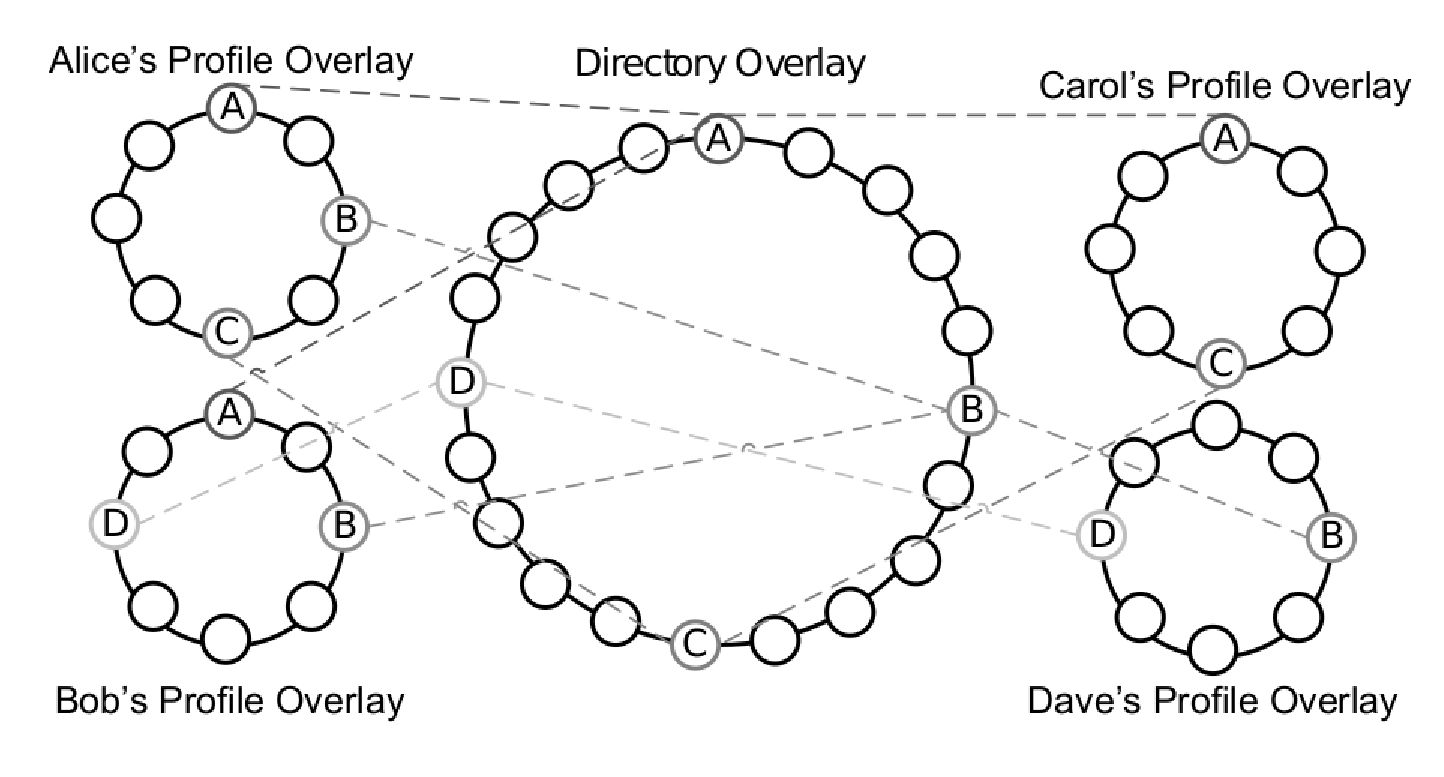
\epsfig{file=figs/subrings.eps, width=\textwidth}
\caption[An example OverSoc social overlay network]{An example OverSoc social
overlay network.  Alice has a friendship with Bob and Carol, hence both are
members of her profile overlay. Bob has a friendship with Alice and Dave but
not Carol; hence Alice and Dave are members of his profile overlay, while Carol
is not.  Each peer has many overlay memberships but a single root represented
by dashed lines in various shades of gray.  For clarity, overlay shortcut
connections are not shown.}
\label{fig:spo.system}
\end{figure}

The rest of this chapter is organized as follows.  Section~\ref{vpo:background}
discusses related work.  Section~\ref{vpo:social_overlays} describes OverSoc,
explaining how to map social networks onto structured P2P overlays.
Section~\ref{vpo:user_interaction} expresses expectations for user interaction in
the system.  In Section~\ref{vpo:outstanding}, I explore some of the remaining
challenges introduced by this approach.  

\section{Related Works}
\label{vpo:background}

In~\cite{peerson}, Buchegger et al. describe how to use a DHT to store social
networking profile.  The DHT provides look-up services for storing meta-data
pertaining to a peer's profile.  Peers query the DHT for updated content from
their friends by hashing their unique identifiers (e.g. friends' email
addresses).  The retrieved meta-data contains information for obtaining the
profile data such as IP address and file version. Their work relies on a PKI
system that provides identification, encryption, and access control.  In
contrast, OverSoc maps individual user profiles and groups to a private overlay
secured by point-to-point encryption and authentication amongst all peers in
the overlay.  The private overlay provides a clean abstraction of access
control, whereby once admitted to a private overlay, users can access a
distributed data store which holds the contents of the owner's profile.

Shakimov et al. in \cite{vis-a-vis} take a different approach by depending on
virtual individual servers (VIS) hosted on a cloud infrastructure such as
Amazon EC2. Friends contact each other's VIS directly for updates.  A DHT is
used as a directory for groups and interest-based searches. Their approach
assumes bidirectional end-to-end connectivity between each VIS, where a profile
is only available during the up time of the VIS.  Because of the demands on
network connectivity and up time, the approach assumes a cloud-hosted VIS and
has difficulty being used on user-owned resources.  OverSoc allows peers to
have  asymmetric connectivity and does not require constant up time through the
use of NAT traversal support and the ability to store the profile in the
overlay's distributed data store.

The approach presented by Cutillo et al. in~\cite{matryoshka} relies on a
central system to host identities and certificates that can then be used to
query a DHT to discover an initial hop in a route to a specific peer through
their circle of friends.  The circle of friends consists of an unstructured
overlay, where direct friends maintain direct connections with the peer, and
outer circles consist of friends of friends and friends of friends of friends.
The main goal of this work is to remove the private components of a profile
from a central entity, whereas OverSoc makes a clean break from all
centralization and enables scalability through distributed replication
techniques.

Unlike the above approaches, the P2P social network presented by Abbas et al.
in~\cite{tribler-osn} uses an unstructured overlay without a DHT where peers
connect directly to each other rather than through the overlay establishing
unique identifiers to deal with dynamic IPs.  Peers cache each other's data to
improve availability, while helper nodes are used to assist with communication
between peers behind NATs.  The approach lacks security and access control
considerations and lacks the guarantees and the simplicity of the abstraction
offered by a structured overlay.

\begin{figure}
\centering
\epsfig{file=figs/friendship_request.eps, width=\textwidth}
\caption{Alice requests and receives a friendship from Bob.}
\label{fig:friend_request}
\end{figure}

\section{Social Overlays}
\label{vpo:social_overlays}

In this section, I explain how OverSoc maps online social networking to virtual
private overlays consisting of a public directory overlay with many private
profile overlays.  The directory overlay supports friend discovery and
verification and stores a lists of peers currently active in each profile
overlay.  Profile overlays support message boards, private messages, and media
sharing.

\subsection{Finding Friends}

In a traditional social network, directories are used to search for users based
upon public information, such as the user's full name, user ID, e-mail address,
group affiliations, and friends.  The resulting search returns zero or more
matching directory entries.  In OverSoc, directory entries are inserted into
the DHT of a public overlay.  Since the public information has many components,
various subsets form DHT keys that all point to a common, complete listing of
the matching public information.  For example, a user can store a pointer at
the DHT key $hash("alice")$ or $hash("alice bob")$.  The key here is that any
subset of the user's public information in lower-case format can be hashed into
a DHT index that would eventually direct the searching user to one or more
users' public information.  More explicit searches could sift through the
results and present to the user only those peers matching all the search
parameters.  The amount of information shared publicly should be configurable
by the user.

While looking for an individual, a peer may discover that many individuals have
overlapping public information components, such as the user's name.  Assuming
all entries are legitimate, the overlay must have some method of supporting
multiple, distinct values at the same key, requiring the application and user
to parse the responses and determine the best match by reviewing the contents
of each certificate.  Alternatively, a technique like Sword~\cite{sword}, which
supports attribute based searching, could be used to efficiently find peers in
an overlay.

To address trust levels when searching for friends, a PGP certificate can be
used to store user's public information and verify user's friends and groups.
In OverSoc, the main portion of a PGP certificate contains information such as
user name, full name, e-mail address, potentially other user-defined data, and
signature packets from the user and those that trust the certificate including
groups and individuals.  These signature packets represent a list of verifiable
friends and groups assisting to further uniquely identify a user.  Each time a
user befriends someone, they should exchange signature packets containing at a
minimum the friend's PGP certificate ID, a signature expiration time, and a
signature binding this information with the new friend's existing PGP
certificate.  This increases the trust level of individuals searching for
others especially if they have common friendships or group membership.  The use
of a time stamp in the signature assists in deciding whether or not a
friendship link is still active without accessing the profile overlay of either
peers.  Thus peers that maintain friendships need to periodically exchange
signature packets.

\begin{figure}
\centering
\epsfig{file=figs/friendship_join.eps, width=\textwidth}
\caption{Alice, already a friend of Bob, connects to his social overlay.}
\label{fig:friendship_join}
\end{figure}

\subsection{Making Friends}

In this example, Alice becomes friends with Bob, as illustrated in Figure
\ref{fig:friend_request}.  Once a user, \textit{Alice}, has found a friend
candidate, \textit{Bob}, \textit{Alice} can issue a friendship request and
store it in the DHT using the hash of Bob's certificate as an index, this acts
a public overlay mailbox.  \textit{Bob} can review the public information of
\textit{Alice} prior to making a decision.  If \textit{Bob} accepts the
request, \textit{Alice} and \textit{Bob} exchange signature packets and are
granted access to each other's profiles.  Once profile access has been enabled,
the \textit{Alice} and \textit{Bob} can learn more information, and if it turns
out to be a mistake, either one of them can unilaterally end the relationship.

Alice's friendship request should contain a pointer to her certificate in the
overlay, a time stamp, and Bob's certificate identifier.  The friendship
request is encrypted using Bob's public key and signed using Alice's private
key for the purposes of anonymity and authenticity.  When Bob receives the
friendship request, he can verify that the request was made for Bob by Alice.
Upon receiving the friendship request, he has three choices:  a conditional
accept, an unconditional accept, or a reject.  During an unconditional accept,
Bob signs Alice's PGP certificate and issues a request to befriend her.
Alternatively, he could issue a request to befriend her and wait for her to
sign his certificate and investigates her profile prior to signing hers.

Discovery of a user is not limited to the directory entries.  Because users
have a public overlay based mailbox, they are not required to discover each
other only through the directory.  Instead, they can use out of band discovery,
using mechanisms like e-mail, chat, or personal websites to exchange
certificates.  Once a peer has received another peer's certificate, they can
submit secure friendship requests using the public overlay.  In fact, this sort
of system can leverage the trust established by an existing social network to
sign and exchange OverSoc's certificates.  

\subsection{The Profile Overlay}
\label{vpo:profile_overlay}

In a traditional social network, the profile or user-centric portion consists
of private messaging, data sharing, friendship maintenance, and a public
message board for status updates or public messages.  In this section, we
explain how these components can be applied to a structured overlay dedicated
to an individual profile.

Using the techniques such as those described earlier, it is feasible to
efficiently multiplex a P2P system across multiple, virtual private overlays
enabling each profile owner to have a profile overlay consisting of their
online friends.  For access control, OverSoc employs point-to-point encryption
and authentication, peers bootstrap private connections by exchanging the base
of the PGP certificate and the profile overlays signature packet obtained in
the ``making friends'' stage.  Because the profile owner also is the CA,
control of which could be distributed across the users resources, for all
members of the overlay, they can easily revoke users from access to the profile
overlay.  Chapter~\ref{chap:security} describes efficient mechanisms for
overlay revocation through the use of broadcasting for immediate revocation and
the use of DHT for indirect and permanent revocation.

The message board of a profile can be stored in two ways: distributed within
the profile overlay via a data store or stored on the profile owner's personal
computing devices.  The distributed data store provides the profile when the
owner is offline and also distributes the load for popular profiles.  For
higher availability, each peer always stores and provides all data in their
profile when they are online.  To ensure authenticity and integrity, peers sign
their messages and each peer's certificate is available in the overlay as well
as stored by mutual friends for verification.  Messages that are unsigned are
ignored by all members of the overlay.  An ideal overlay for this purpose
should support complex queries~\cite{complex_queries} allowing easy access to
data stored chronologically, by content, by type, i.e., media, status updates,
or message board discussions.

Private messaging in the profile overlay is unidirectional; only the profile
owner can receive private messages using their overlay.  To enforce this, a
private message should be prepended with a symmetric key encrypted by the
profile owners public key, the message should be appended by a signature of the
message using the private key of the message sender, and the entire message
encrypted by the symmetric key.  This approach ensures that only the sender and
the profile owner can decrypt the private message and verify the senders
identity.  The contents of the private message include the sender, time sent,
and the subject.  Messages are be stored in well known locations in the DHT,
like ``private messages for me'', so that the profile owner can either poll the
location.

\subsection{Event Based Message Notification}

Both the directory and profile overlays have methods by which peers can receive
messages.  In the directory overlay, these take form by means of friendship
requests and friendship accepts, certificate signature packets.  The profile
overlay supports private messages.  While polling the location in the DHT
occasionally will allow peers to receive the messages, polling has inherent
delays and network costs.  Alternatively, event  enable peers to receive sent
messages very quickly after they have been sent with minimal impact on network
throughput.

A simple method for implementing an event notification system involves using
the DHT.  Each event would have an identification that would map to a list of
peers wanting to know when an event occurred and the data associated with it.
Thus mapping the $(event id, listener)$ to the DHT could be done by hashing a
string such as ``private messages for me'' or taking a hash of the user's
certificate hash for public overlay messages and storing the profile owners
active nodes into the list of listeners .  When a message is inserted into the
user's mailbox, the sender could query this list and send to each listener a
notification of the new private message.  Alternatively, if a higher degree of
anonymity is required, the DHT server could be modified to forward the response
to the listeners directly rather than returning a list of listeners.  Of
course, this does not prevent potential race conditions occurring, such as a
situation where a peer recently joined their profile overlay, had already
queried their mailbox and found it empty, while simultaneously a private
message was sent to them yet they were not in the listeners list.  Thus
occasional polling is required, though can be minimized, the longer a node has
been online.

\subsection{Active Peers}

The directory overlay should be used to assist in finding currently active
peers in the profile overlays.  By placing their node IDs at a well-known,
unique per-profile overlay keys in the DHT, active peers can bootstrap incoming
peers into the profile overlay.  I implemented and evaluated this concept in
Chapter~\ref{chap:security}.  Because the profile overlay members all use PKI
to ensure membership, even if malicious peers insert their ID into the active
list, it would be useless as the peer would only form connections with peers
who also have a signed certificate.  Extending from the earlier example, where
Alice became Bob's friends, Figure~\ref{fig:friendship_join} presents in detail
how she would join his private overlay.

\subsection{Groups}

Groups can be considered extensions of profile overlays.  The fundamental
difference between a group and a profile is that a group lacks private
messaging and has shared ownership.  So just as a peer can find a profile in
the directory by hashing the name of the user and other identifiable
information, so can the user find the group.  Like the certificate of the user,
the members of a group sign the group's certificate to represent their
membership to that group.  In OverSoc, users request membership to the group
like they do friendship requests, in response a group manager can sign their
certificate allowing that member access to the group.  Finally, the group can
be bootstrapped in the same way as the profile overlay through the directory
overlay.

The unique challenge presented by groups is the sharing of the CA task.  A
decentralized solution would be for all members of the group to be listed in
the groups DHT and when a peer becomes a manager, they obtain a new signature
packet that contains a user-defined component stating that they are managers.
If an administrator loses their position, then all members who had their
certificate signed by that administrator would need to obtain a new
certificate.  To avoid member churn, the owner could provide signature packets
for all group members.  Thus the managers just allow temporary access until the
owner comes online and provides more permanent access.

\section{User Interaction}
\label{vpo:user_interaction}

OverSoc consists of many components that are transparent to the user, the user
experience should appear to the user no differently than an existing online
social network.  The OverSoc could be a downloadable application or a browser
based Flash or Silverlight application.  If the user, Bob, had already created
an account, Bob would be presented with an interface showing their friends
profiles.  Based upon Bob's configuration, the social application could
retrieve profile updates as he navigates to individual profiles or as soon as
the application joins an individual profile overlay, reactive versus proactive
profile querying.  

If this was Bob's first time starting OverSoc, he would be presented with
screens asking for his privacy preferences, such as whether or not he wants his
information in the directory overlay, if he felt comfortable enough with the
idea of people knowing he was a member of the social network and who his
friends are.  Then OverSoc would ask for personal information to populate his
profile and to generate his directory information.  At which point, the OverSoc
would join the overlay and create Bob's private overlay.  Bob could then start
searching for friends, make friend requests, and respond to friend requests.

Recently, Bob had been thinking about his high school days and was curious if
Alice was also a member of OverSoc, though Bob did not have Alice's e-mail
address, just her first and last name.  Bob enters Alice's name into the
OverSoc search box and is presented by a list of Alice's.  As Bob reviews each
of the entries, he recognizes an Alice that is friend's with some of the same
people Bob was in high school.  Bob selects to become her friend.  At which
point, the OverSoc transparently inserts a friendship request to Alice and
signs Alice's certificate so Alice can view Bob's profile.  Of course that is
because Bob has chosen to allow user-initiated friend requests access to his
profile.  Alice receives Bob's request, peruses his profile and feels fine
becoming friends with Bob, which initiates a transparent process of signing
Bob's certificate and placing the result in the public overlay.  There is one
problem though, when Bob receives Alice's signature and views her profile, he
realizes that this is some other Alice.  He quickly chooses to defriend her.
This causes Bob's OverSoc instance to broadcast a revocation for Alice's
signature and to store the revocation in the DHT.  Alice, who was viewing Bob's
profile, is notified of this sudden loss of trust and while she is able to view
the contents of Bob's profile, which she has already accessed and obtained, she
can no longer receive updates as members of Bob's overlay prevent her from
accessing it.

In another instance, Bob bumped into Carol, who e-mailed Bob a copy of her
certificate.  Bob points OverSoc to the certificate, and OverSoc verifies that
he wants to become friends with the identity associated with the certificate.
When he accepts, OverSoc immediately submits a request to become Carol's
friend.  Carol receives notification and accepts Bob's friendship request.  At
this point, both Bob and Carol have transparently exchanged signed certificates
and have mutual access to each other profiles.  As Bob reads Carol's latest
news, he remembers a funny personal story and that he would like to share with
Carol.  So he sends Carol a private message.  Carol is offline though.  The
next time Carol goes online, her social application discovers the message and
presents it to her.  In this scenario, OverSoc  has taken the private message,
secured it with her public key and a symmetric key and signed it with his
private key.  After which, it inserts the message into the DHT and sends a
notice to the event notification system, which detects that there were no
listeners.  When Carol's application comes online, it queries the DHT receiving
the message.  Prior to presenting Carol the message, the OverSoc decrypts and
verifies the message.

The OverSoc architecture can leverage existing social networks to bootstrap
trust.  For example, consider Bob and David are two friends on Facebook.  Bob
joins a Facebook application called ``OverSoc/Facebook Bridge'', which stores
a copy of his OverSoc certificate in his personal profile.  Bob has been
bragging to David about OverSoc and mentions to him how easy it is to migrate
from Facebook to OverSoc using this application.  So David joins OverSoc as
well as the application.  When David accesses the application, it pastes his
certificate to his profile, notifies notifies him that he has a friend already
using it, Bob, and that he can immediately sign Bob's certificate, and leaves a
request for Bob to sign his certificate.  Additionally, when David logs into
OverSoc, he can leave a friend request there as well, so that the next time
Bob accesses Facebook or OverSoc, he will receive David's request and can sign
David's certificate.  At which point, both will have access to each others
OverSoc profile overlays.  

\section{Challenges}
\label{vpo:outstanding}

While structured P2P overlays have been well-studied in a variety of
applications, their use in social profile overlays raises new interesting
questions, including:

{\bf 1) Handling small overlay networks} - P2P overlay research typically
focuses on networks larger than the typical user's friend count (Facebook's
average is 130\footnote{http://www.facebook.com/press/info.php?statistics}).
Because social profile overlays are comparatively smaller, this can impact the
reliability of the overlay and availability of profile data.  A user can host
their own profile; however when the user is disconnected it is important that
their profile remains available even under churn. It is thus important to
characterize churn in this application to understand how to best approach this
problem. An optional of per-user deployment of a virtual individual server
(VIS) and the use of replication schemes aware of a user's resources provide
possible directions to address this issue.

{\bf 2) Overlay support for low throughput, unconnected devices} - devices such
as smart phones cannot constantly be actively connected to the overlay and the
connection time necessary to retrieve something like a phone number may be too
much to make this approach useful.  Similar to the previous challenge, this
approach could benefit from using a VIS enabling users access to their social
overlays by proxy without establishing a direct connection to the overlay
network.

{\bf 3) Reliability of the directory and profile overlay} - Overlays are
susceptible to attacks that can nullify their usefulness.  While the profile
overlay does have point-to-point security, in the public, directory overlay,
the lack of any form centralization makes policing the system a complicated
procedure.  While the approach of appending friends list can assist users in
making decisions on identity, it does not protect against denial of service
attacks.  For example, users could attempt create many similar identities in an
attempt to overwhelm a user in their attempt to find a specific peer.  Previous
work has proposed methods to ensure the usability of overlays even while under
attack.  For the social overlay to be successful, one must identify which
methods should be used. A possible approach is to replicate public information
within a user's profile overlay thus providing an alternative directory overlay
for querying prior to using the public directory overlay.

{\bf 4) Social profile data storage} - In previous works, DHTs have been used
as the building blocks to form more complex distributed data stores as
presented in Past~\cite{past} and Kosha~\cite{kosha}.  Application of data
stores will be heavily dependent on the churn rate associated with the overlay.
If the system lacks any reasonably stable membership, large data files may be
corrupted while smaller data sets are completely lost.  Ideally, the usage
model would be similar to those of Skype and Twitter, which have active
processes for the duration of the computers usage.  In an environment like
this, data storage would be limited only by the available bandwidth of the
participants.
